\documentclass{article}

% if you need to pass options to natbib, use, e.g.:
% \PassOptionsToPackage{numbers, compress}{natbib}
% before loading nips_2016
%
% to avoid loading the natbib package, add option nonatbib:
% \usepackage[nonatbib]{nips_2016}

\usepackage[final]{nips_2016}

% to compile a camera-ready version, add the [final] option, e.g.:
% \usepackage[final]{nips_2016}

\usepackage[utf8]{inputenc} % allow utf-8 input
\usepackage[T1]{fontenc}    % use 8-bit T1 fonts
\usepackage{hyperref}       % hyperlinks
\usepackage{url}            % simple URL typesetting
\usepackage{booktabs}       % professional-quality tables
\usepackage{amsfonts}       % blackboard math symbols
\usepackage{nicefrac}       % compact symbols for 1/2, etc.
\usepackage{microtype}      % microtypography
\usepackage{graphicx}


\makeatletter

\title{Moral Reasoning Classification in Law}

% The \author macro works with any number of authors. There are two
% commands used to separate the names and addresses of multiple
% authors: \And and \AND.
%
% Using \And between authors leaves it to LaTeX to determine where to
% break the lines. Using \AND forces a line break at that point. So,
% if LaTeX puts 3 of 4 authors names on the first line, and the last
% on the second line, try using \AND instead of \And before the third
% author name.

\author{
  Nischal Mainali\\
  NYU Abu Dhabi\\
  \texttt{nischal.mainali@nyu.edu} \\
  %% examples of more authors
 \And
  Liam Meier\\
  NYU Abu Dhabi \\
  %% Address \\
  \texttt{liam.meier@nyu.edu} \\
   \AND
  Elliot Ash\\
  Assistant Professor of Economics\\
  University of Warwick\\
  \texttt{elliott.t.ash@gmail.com} \\
   \And
  Daniel Chen\\
  Professor \\
  Toulouse School of Economics\\
  \texttt{daniel.li.chen@gmail.com} \\
  %% \AND
  %% Coauthor \\
  %% Affiliation \\
  %% Address \\
  %% \texttt{email} \\
  %% \And
  %% Coauthor \\
  %% Affiliation \\
  %% Address \\
  %% \texttt{email} \\
  %% \And
  %% Coauthor \\
  %% Affiliation \\
  %% Address \\
  %% \texttt{email} \\
}


\begin{document}
% \nipsfinalcopy is no longer used

\maketitle

\begin{abstract}
We build a Linear-SVM classifier for moral reasoning, training on articles of philosophers reasoning about the morality of various issues from consequentialist and deontological positions. We then apply this classifier to circuit court opinions to understand trends in moral reasoning.

\end{abstract}



\section{Introduction: Question and Approach}
How do we reason morally? Broadly, the two broad categories of moral frameworks that philosophers most often consider  are consequentialist and deontological frameworks.

For a consequentialist, what one ought to do is whatever brings about the best consequences. The most famous form of consequentialism is utilitarianism, according to which agents are obligated to do whatever brings about the most utility. For hedonist utilitarians like J.S. Mill and Jeremy Bentham, pain is bad and pleasure is good. Other philosophers have argued for other conceptions of utility.

In a deontological framework, an act is right if it conforms to a moral norm. For Kant, this is the categorical imperative, the first formulation of which holds that one should act only according to a maxim which they can will to be a universal law.

Applied ethicists argue about the morality of various issues from these positions. Take the permissibility of lying, for example. A consequentialist might argue that it would be permissible to lie if the consequences of telling the lie would be better than not telling the lie. In contrast, typically a deontologist would argue that it's always immoral to lie because one could not will the acting of lying to be a universal law.

Law commonly operates in correspondence with morality. Some actions are made illegal not because of practical considerations, but because a society reasons that the action is wrong.

In the legal system, we can observe when judges  reason according to either of these moral frameworks. In the case of a contract, a judge reasoning deontolgically may hold that there can be not just breach of the contract. A judge reasoning consequentially may reason that certain breaches of contract are acceptable, if, for example, a breach of contract would lead to a better outcome for the relevant parties.

We attempt to build a classifier using the tools of machine learning to identify these cases of moral reasoning. To train our classifier, we use the texts of articles in the applied ethics literature, where various philosophers argue about issues such as abortion, vegetarianism, and war from consequentialist and deontological stances. We then apply our classifier to circuit court opinions, where judges outline their reasoning for their decision on a case.

We use these opinions provide a proxy for identifying trends in moral reasoning in the United States. With our circuit court data dating back to 1883, we can identify trends in moral reasoning. We look at rates of consequentialist vs deontological reasoning over time, according to where the individual was born, where the individual attended school, their sex, and the party of the president under which they were nominated.

\section{Dataset}
For the training data, we collect all the philosophy paper database PhilPapers.org tagged with “Applied Consequentialism” or “Applied Deontology”. After filtering out papers written in other languages, papers that had both consequentialism and deontology tags, and papers that obviously didn’t belong, we were left with 14 Consequentialist papers and 11 Deontology papers. These were converted to .txt, and artifacts that were not the text of the paper (Watermarks like “Downloaded from NYU”) were also expunged when possible.

The data we classify were Circuit Court Opinions. These opinions are part of a dataset collected by Daniel Chen and Elliot Ash. Relevant metadata is available, including many biographical details of the judges writing the opinions.

\section{Data preprocessing and Featurization}
Our data set is composed of few large texts. As these most text classification techniques perform better with larger corpa, we separated each of our Consequentialist and Deontology corpa into 100 equally sized chunks. We are aware that this might result in the model memorizing the data sets identity instead of learning right signals. But this can be easily handled by tweaking randomness seed for proper separation of the data set into training and validation set.

Next was featuirizing the text. In the past, varied approached such as bag of words, n-gram, tf-idf and so on for featurizing the text. After some experimentation, we chose tf-idf with n-gram featurization. In essence, we take phrases made up of up to 3-words and adjust them by their document frequency to create a list of tf-idf n-grams. We then vectorized, which in a broad sense is done by PCA (dimensionality reduction) methods. 
\section{Training}
The preprocessing step leaves us with a vector assigned to each of the text that we will use for training the Machine Learning model. Natural choice for classification problems such as ours is Linear Support Vector Machine (SVM) or Naive Bayes. Initial performance of Naive Bayes was very poor, so we focused our efforts on implementation of the SVM.

In broad terms, Linear-SVM tries to find a hyperplane that neatly separates the vectors with 'Deontology' labelling and 'Consequential' labelling. On one side of the hyperplane we find Consequentialist text and on the other side we find deontological texts, and the prediction is through which side of the hyperplane does the vector of the text lies in. 

During the initial steps in the training, we separate our data sets into training and validation set. After each training, the model predicts on the validation set and we tweak the training parameters to increase accuracy and get sensible features. The major tuning component in training the model was frequency threshold and stop words. 

Our model very quickly approached a 100\% prediction accuracy in the validation set, so the main hyperparamenter tuning step was finding junk features in the prediction function and removing them. For example: “New York University”, because some of the PDFs were downloaded on an NYU license, which appears on each page of text in some of the documents, other overfitting type terms (e.g. “fetus”), and high frequency junk phrases such as 'x-86'. 

We did this by examining the prediction function. Linear-SVM predicts by assigning weights (coefficients) to the n-grams. So, we looked at the top 50 predictors for both Consequentialist reasoning and Deontological reasoning and weeded out irrelevant n-grams. 

We also experimented with n-grams by adjusting the number of words per phrase. 3 words gave a strong result and increasing it further helped very little, if any, at the risk of creating overfit features.


\section{Prediction Function}

\subsection{Prominent n-grams}

The end product of the training is a weight assigned to each of the n-gram in the feature. We rank the n-grams by their weights. An n-gram with a positive weight means that it signals that a the text is deontological, and similarly negative weight signals that the text is consequentialist.

\subsubsection{Consequentialist n-grams}
\begin{center}
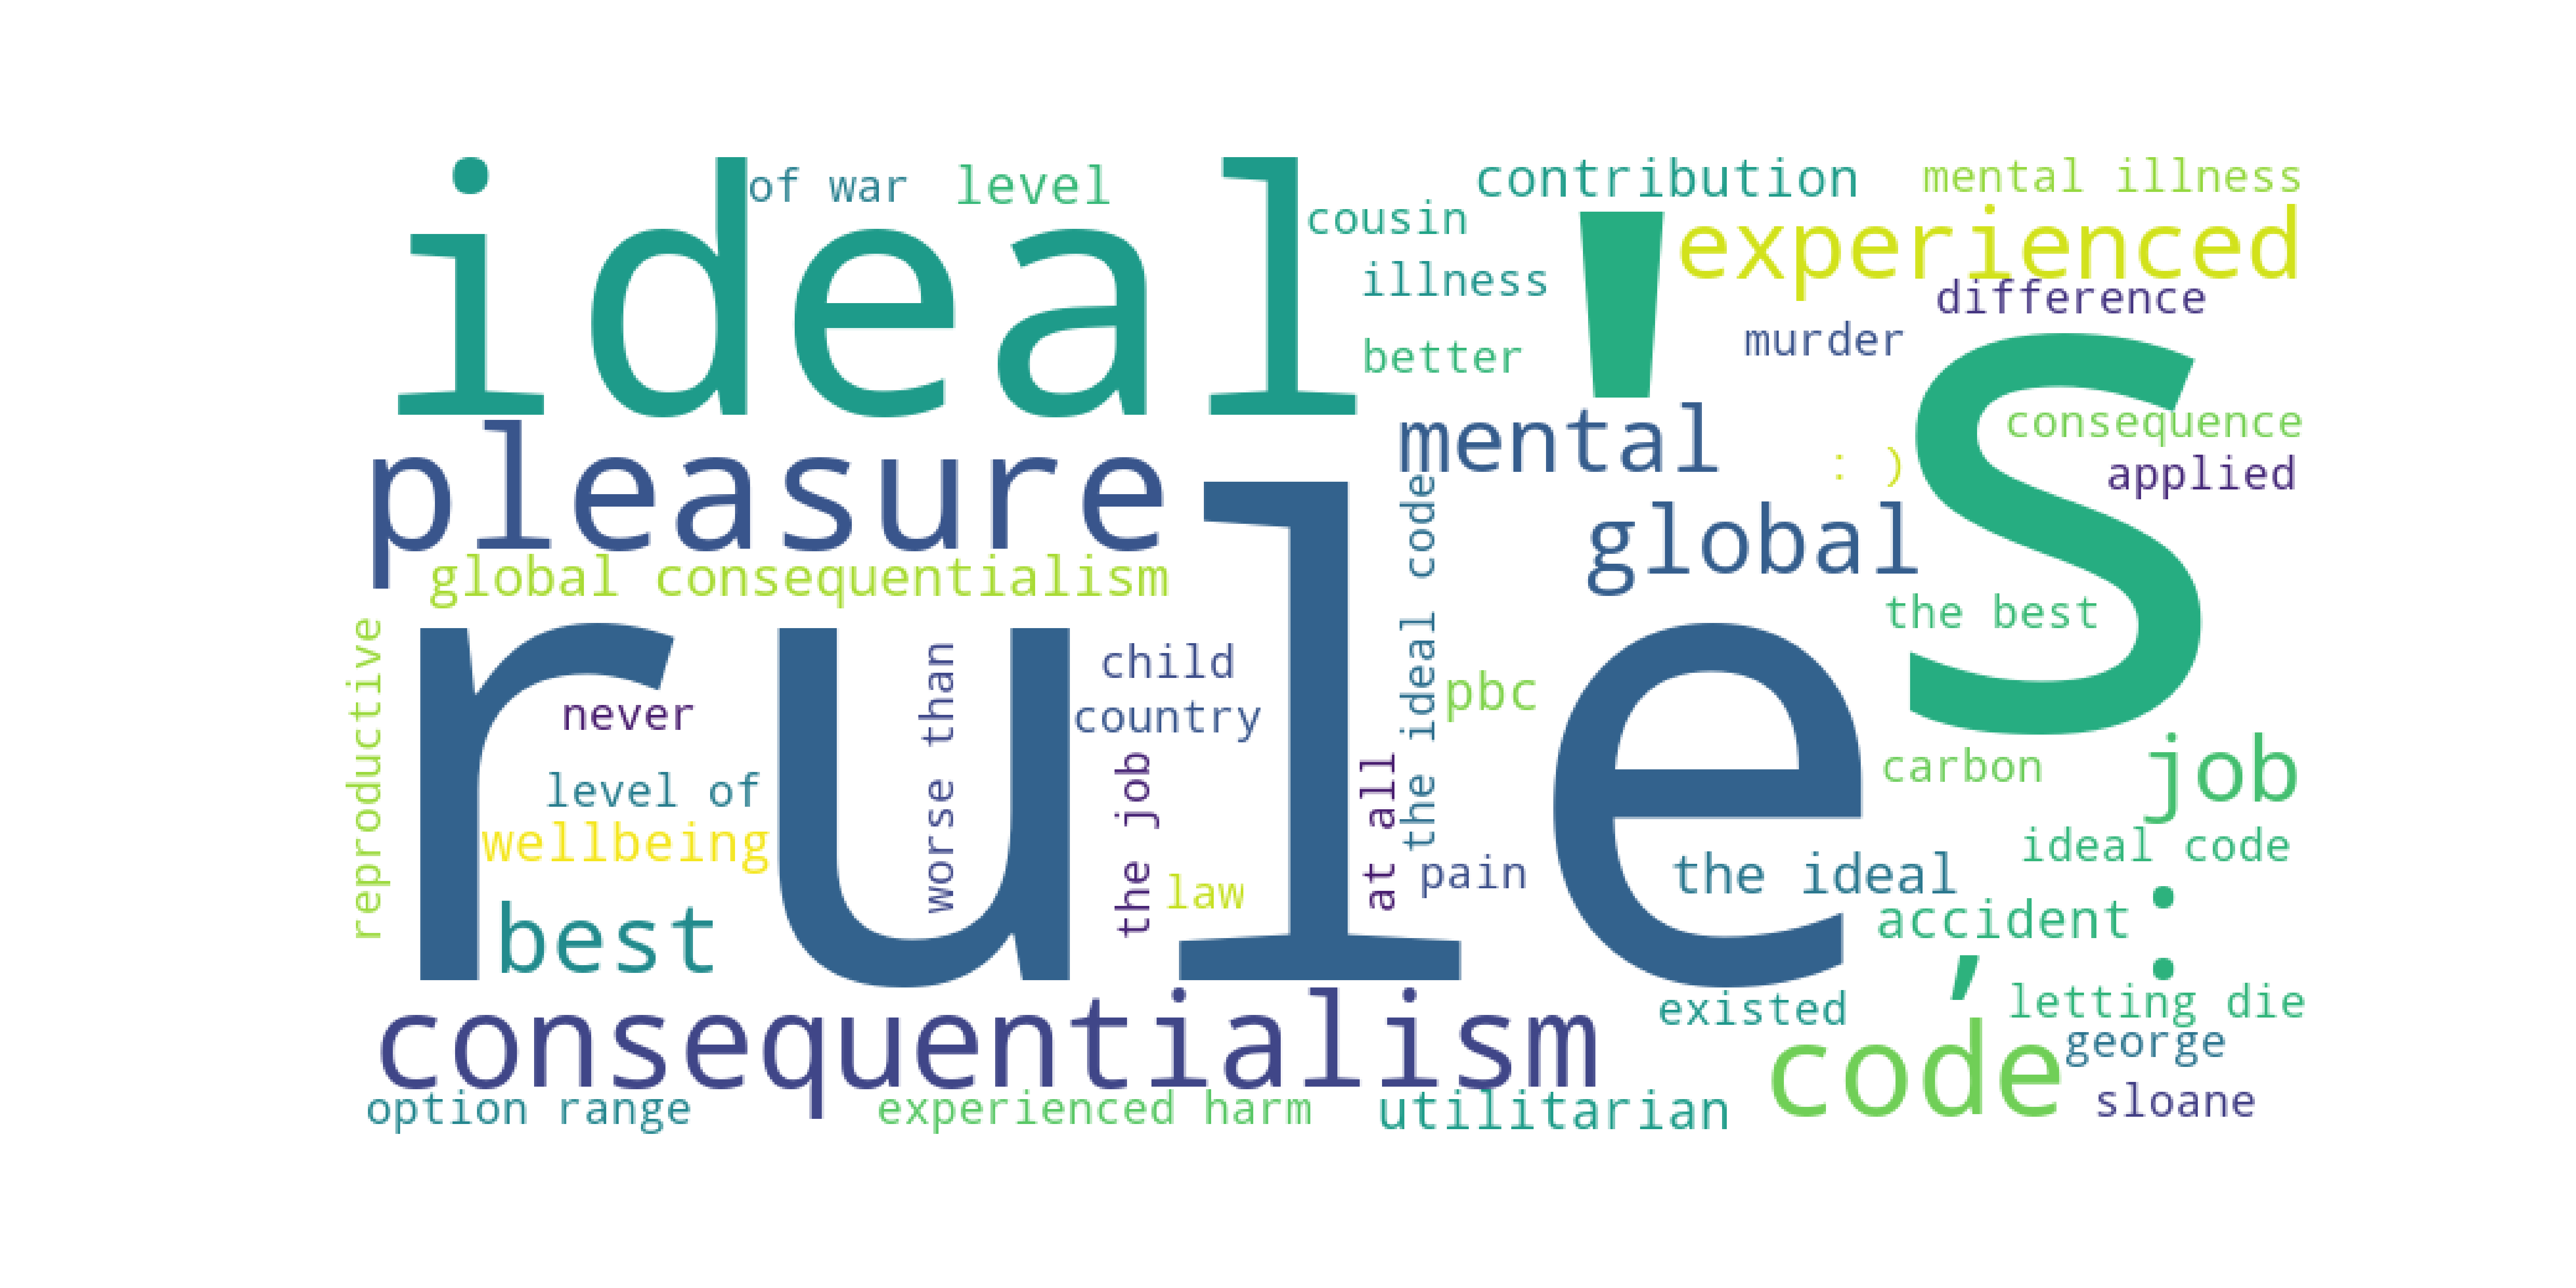
\includegraphics[width = 16cm] {cons_cloud.png}
    \[\texttt{Consequentialist Word Cloud}\]
\end{center}

\subsubsection{Deontological n-grams}
\begin{center}
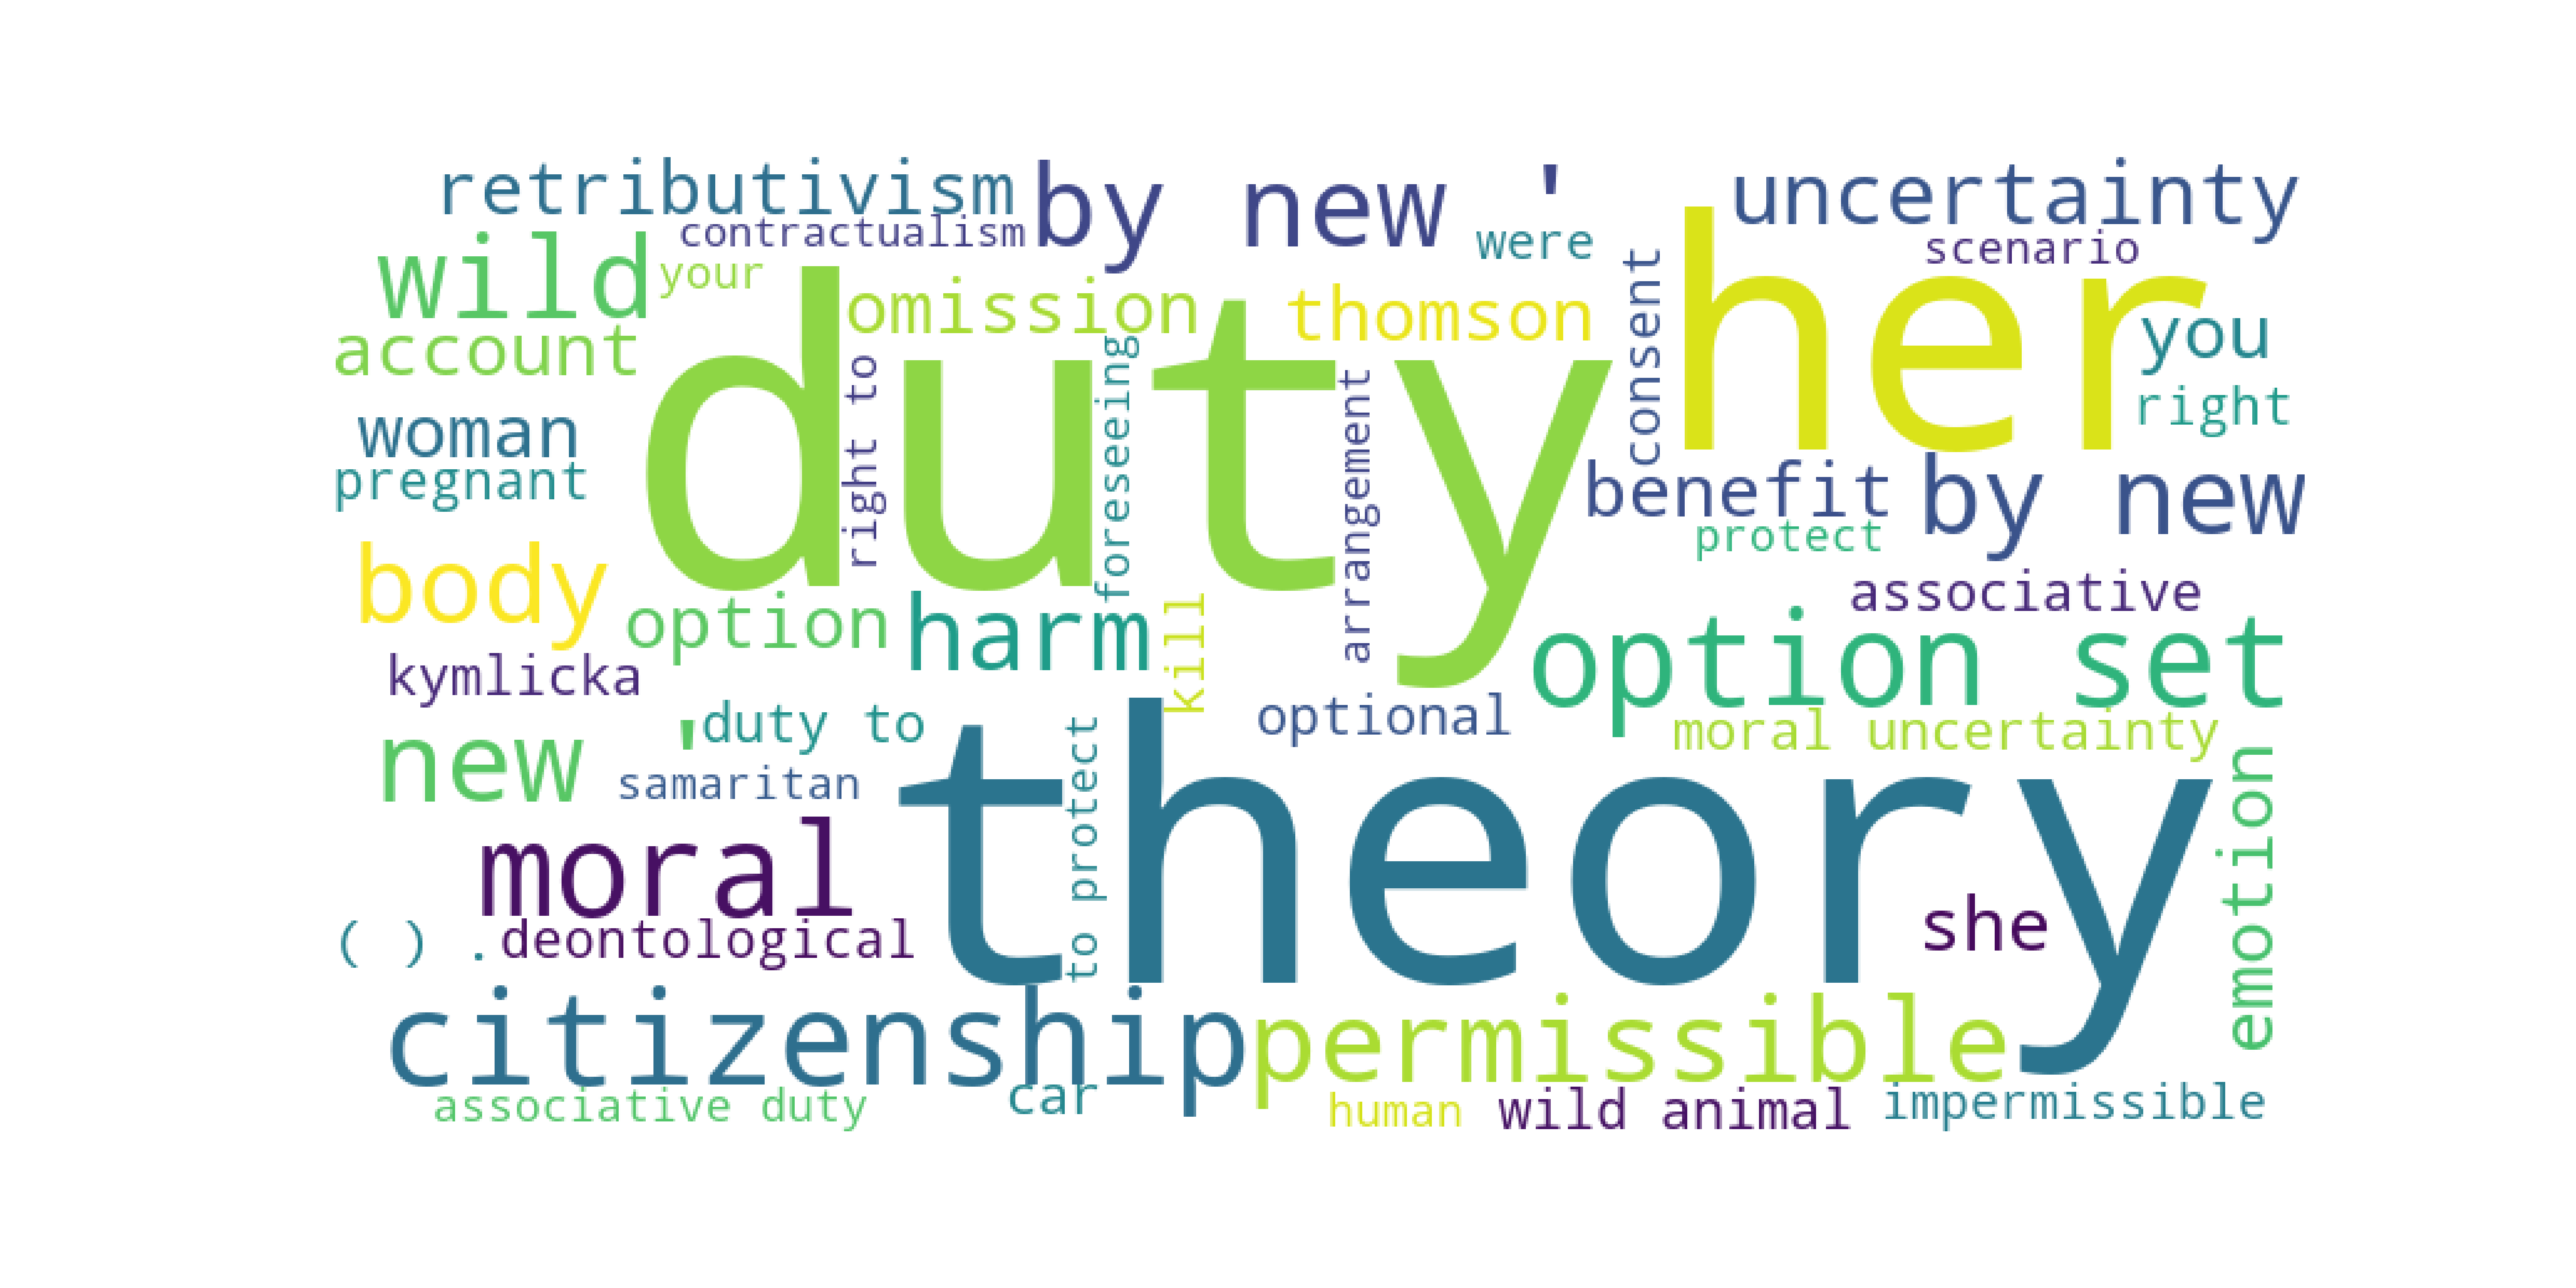
\includegraphics[width = 16cm]{deon_cloud.png}
    \[\texttt{Deontological Word Cloud}\]
\end{center}

\subsection{Prominent Paragraphs}

\subsubsection{Strongly Deontological Prediction}
The following paragraph was considered deontological by the predication function with high confidence: \newline

\begin{enumerate}
    \item 
\texttt{
In contrast, under Oregon insurance law the duty to indemnity is not completely dependant upon the duty to defend. See Ledford v. Gutoski, 319 Or. 397, 403 , 877 P.2d 80, 84 (1994). ("The duty to indemnify is independent of the duty to defend."). Liability for indemnity, unlike liability under the duty to defend, derives from factual determinations separate from the allegations in the complaint. As a result, American could still have a duty to indemnify even if it did not have a duty to defend.
}
    \item
\texttt{
Under FELA, a railroad has a duty to provide its employees with a reasonably safe workplace; this does not mean that a railroad has the duty to eliminate all workplace dangers, but only the "duty of exercising reasonable care to that end." Baltimore & Ohio S.W.R. Co. v. Carroll, 280 U.S. 491, 496, 50 S.Ct. 182, 74 L.Ed. 566 (1930). Grand Trunk does not dispute that it had a duty to exercise reasonable care to protect Van Gorder, an employee. Thus, Van Gorder established the duty component of the negligence standard. Van Gorder cannot, however, show that Grand Trunk breached that duty.
}
    \item
\texttt{
By reason of its nature as a public institution St. Elizabeths Hospital owes a duty to the public in carrying out its difficult responsibilities. We have no occasion now to decide, however, whether its public duty included an entirely separate duty to Mrs. Morgan. There was a particular duty to the Court of General Sessions, and in the circumstances of this case it was intertwined with a duty to her. See infra, note 12.
}
    
    
\end{enumerate}


\subsubsection{Strongly Consequentialist Prediction}
The following paragraph was considered Consequentialist by the predication function with high confidence: \newline
\begin{enumerate}
    \item 
\texttt{
The ALJ's explanation of the reasons for his determination with respect to Cook's psychological impairment seems adequate. He identified the relevant listed impairment, for comparison with Cook's symptoms, as section 12.04, "functional nonpsychotic disorders." He also made a relatively careful comparison of Cook's mental problems with the criteria listed in section 12.04. The evidentiary record on Cook's mental illness is also adequately developed.
}
    \item
\texttt{
The TCCA in the present case repeatedly cited evidence that it interpreted as supporting the existence of Black's mental illness but not of his mental retardation. For example, the TCCA explained that Dr. Engum "believed that Petitioner suffered from personality problems, delusional problems, or psychological difficulties, [but that] those issues are separate and apart from the issue of whether Petitioner was mentally retarded." Black, [2005 BL 43396], 2005 WL 2662577, at *16. The TCCA also concluded, based on Dr. Vaught's testimony, that mental retardation "has nothing, however, to do with mental illness." Id. at *10. This reasoning is similar to the TCCA's error in Coleman of treating "Mr. Coleman's mental illness and intellectual disabilities as separate dichotomous spheres rather than as interwoven causes." Coleman, 341 S.W.3d at 249. On remand, a proper analysis of Black's case under Coleman must consider the potential relationship between mental retardation and mental illness.
}
    \item
\texttt{
I cannot agree that it is so probable that illness or mental illness once experienced continues thenceforth. Common experience is that conditions of illness are changeable, with the exception of physical injuries such as the shortening of a limb, or its loss. Most sick people get better. Many, many mentally ill persons recover and return to productive lives. The fact that someone was mentally ill and in need of psychiatric care five years ago does not mean that they are probably mentally ill today. There are too many persons who have recovered from serious mental breakdowns and become gainfully employed to presume that disability from mental illness ordinarily continues. Indeed, the invalidity of the presumption here is demonstrated by Dr. Harvey's testimony that it is speculative to state what Mr. Richardson's condition was in 1958.
}
    
\end{enumerate}



\section{Analysis}

\subsection{Time Series for Consequentialist Reasoning}
Here, we plot the percentage of consequentialist reasoning over time. There's a swift jump in the 1930s, indicating a major switch in thought at the time. We hypothesize that hardships of the depression brought own moral attitudes that preferred better consequences to strict adherence of standards and law.
\begin{center}
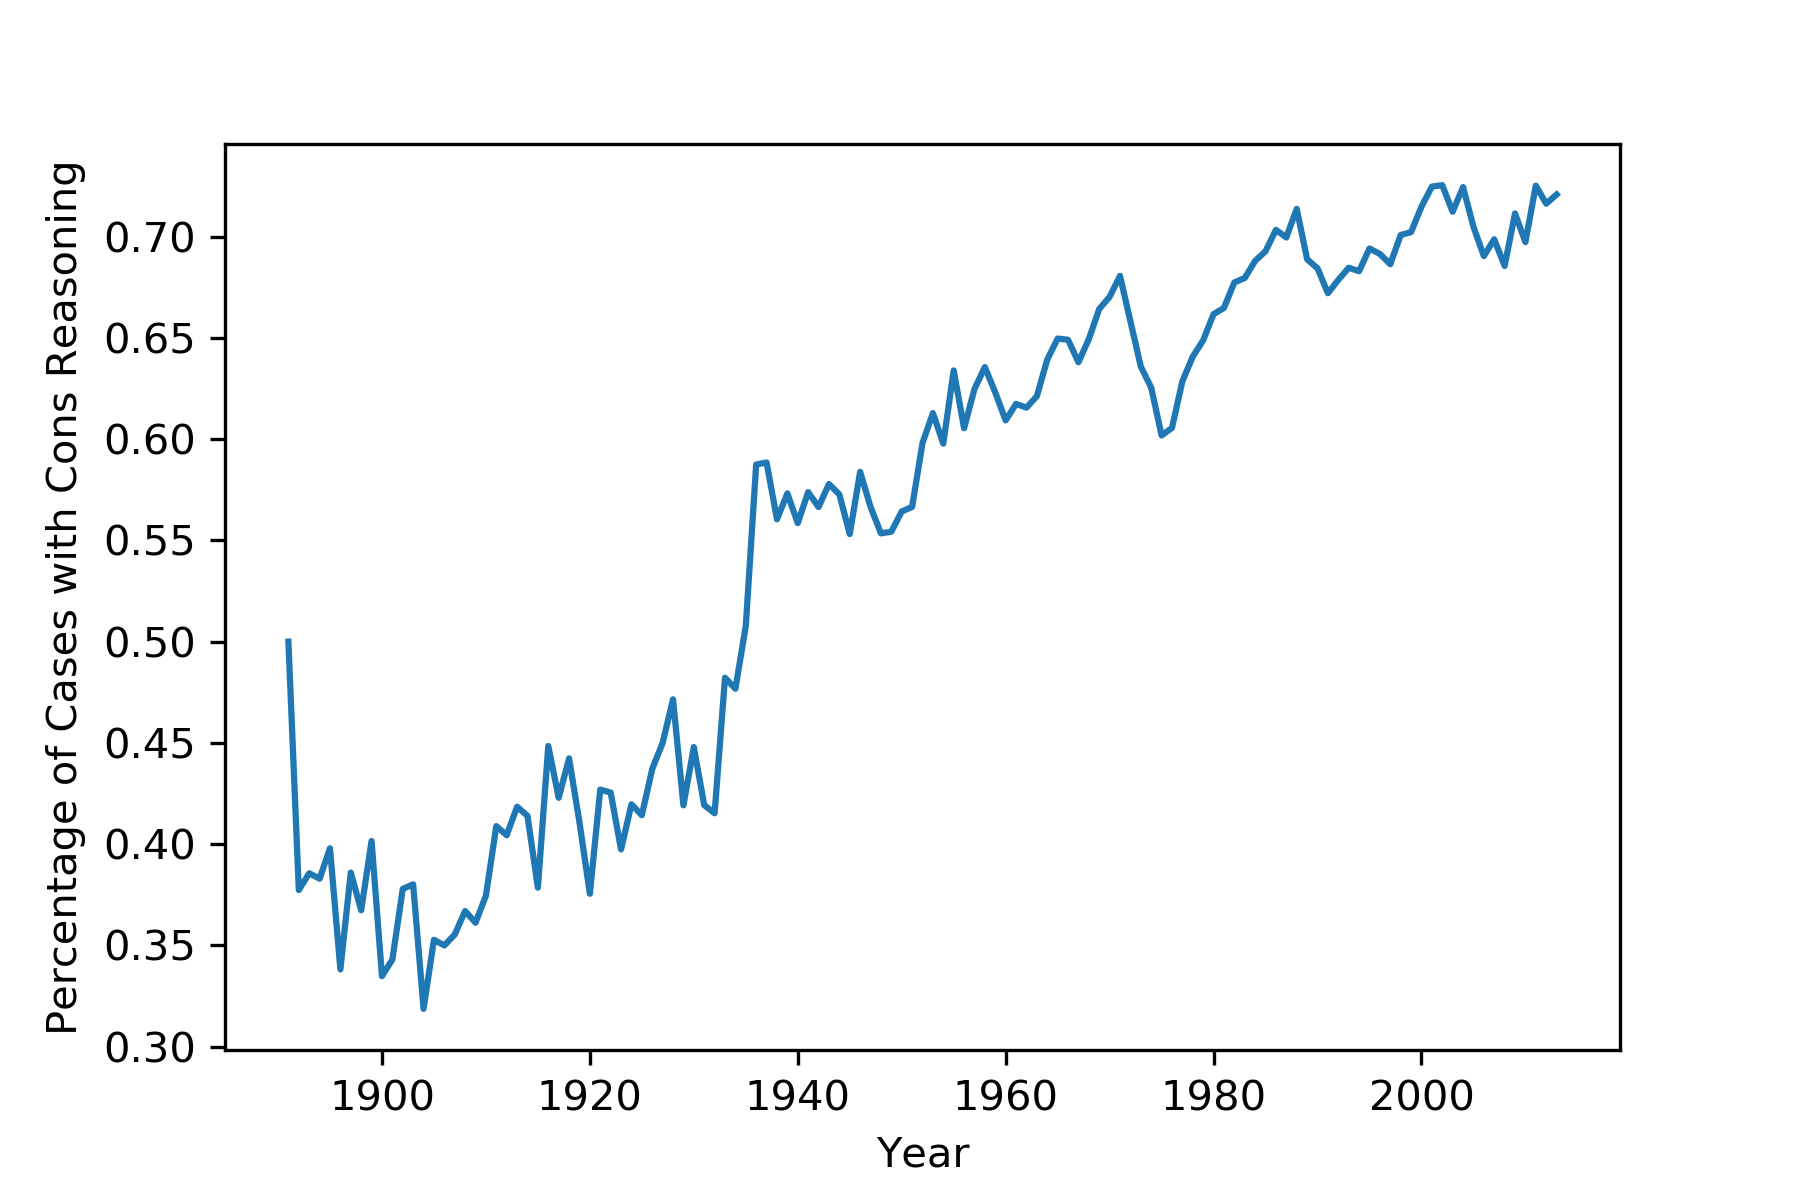
\includegraphics[width = 12cm, height = 8cm]{timeseries.png}
    \[\texttt{Time series 1891 - 2013}\]
\end{center}

\subsection{Majority and Dissenting Opinions in Critical Years}
We plot the percentage of consequentialism in the majority vs dissenting opinions in the years 1920-1932. This indicates that the jump in consequentialist reasoning was preceded by a major dissenting voice of consequentialist reasoning.
\begin{center}
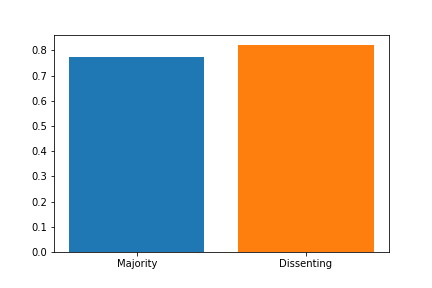
\includegraphics[width = 12cm, height = 8cm]{MajDis.png}
    \[\texttt{Consequentialist reasoning in Majority vs Dissenting Opinion}\]
\end{center}

\subsection{Law School Ranking with Consequentialism Score}
The list below ranks law schools by the percentage of consequentialist reasoning compared to the global average. We only rank schools that yielded above 1000 opinions in our dataset. Above all, the consequentialism dominance in this list indicates that the most proflic schools seem to be leading the back with regard to consequentialist reasoning.
\begin{enumerate}
    \item 'Washington and Lee University School of Law', -19.6\%
    \item 'University of North Carolina School of Law', -9.9\%
    \item 'University of Wisconsin Law School', -9.5\%
    \item 'University of Oxford', -3.5\%
    \item 'University of Nebraska College of Law', 0.5\%
    \item 'St. Louis University School of Law', 1.2\%
    \item 'University of California, Berkeley', 1.7\%
    \item 'New York University School of Law', 2.3\%
    \item 'Columbia Law School', 2.8\%
    \item 'Cornell Law School', 3.1\%
    \item 'Syracuse University College of Law', 3.6\%
    \item 'Fordham University School of Law', 4.0\%
    \item 'University of Arkansas School of Law', 4.3\%
    \item 'University of Alabama School of Law', 4.5\%
    \item 'Harvard Law School', 5.9\%
    \item 'George Washington University Law School', 5.9\%
    \item 'Notre Dame Law School', 6.0\%
    \item 'Northwestern University School of Law', 6.1\%
    \item 'University of Utah College of Law', 7.2\%
    \item 'University of Washington School of Law', 7.4\%
    \item 'University of Southern California Law School', 7.6\%
    \item 'University of Virginia School of Law', 7.8\%
    \item 'Louisiana State University Law School', 8.4\%
    \item 'Yale Law School', 8.4\%
    \item 'University of Minnesota Law School', 8.5\%
    \item 'University of Chicago Law School', 9.6\%
    \item 'Tulane University Law School', 9.6\%
    \item 'University of Texas School of Law', 11.1\%
    \item 'University of Mississippi School of Law', 11.4\%
    \item 'University of Montana School of Law', 11.7\%
    \item 'Stanford Law School', 12.1\%
    \item 'Georgetown University Law Center', 17.2\%
\end{enumerate}

\subsection{Consequentialist approach per Gender}

There seems to be very little difference across gender in moral reasoning. While, it appears that females are more likely to reason consequentially, the difference is too small to be a reliable signal.

\begin{center}
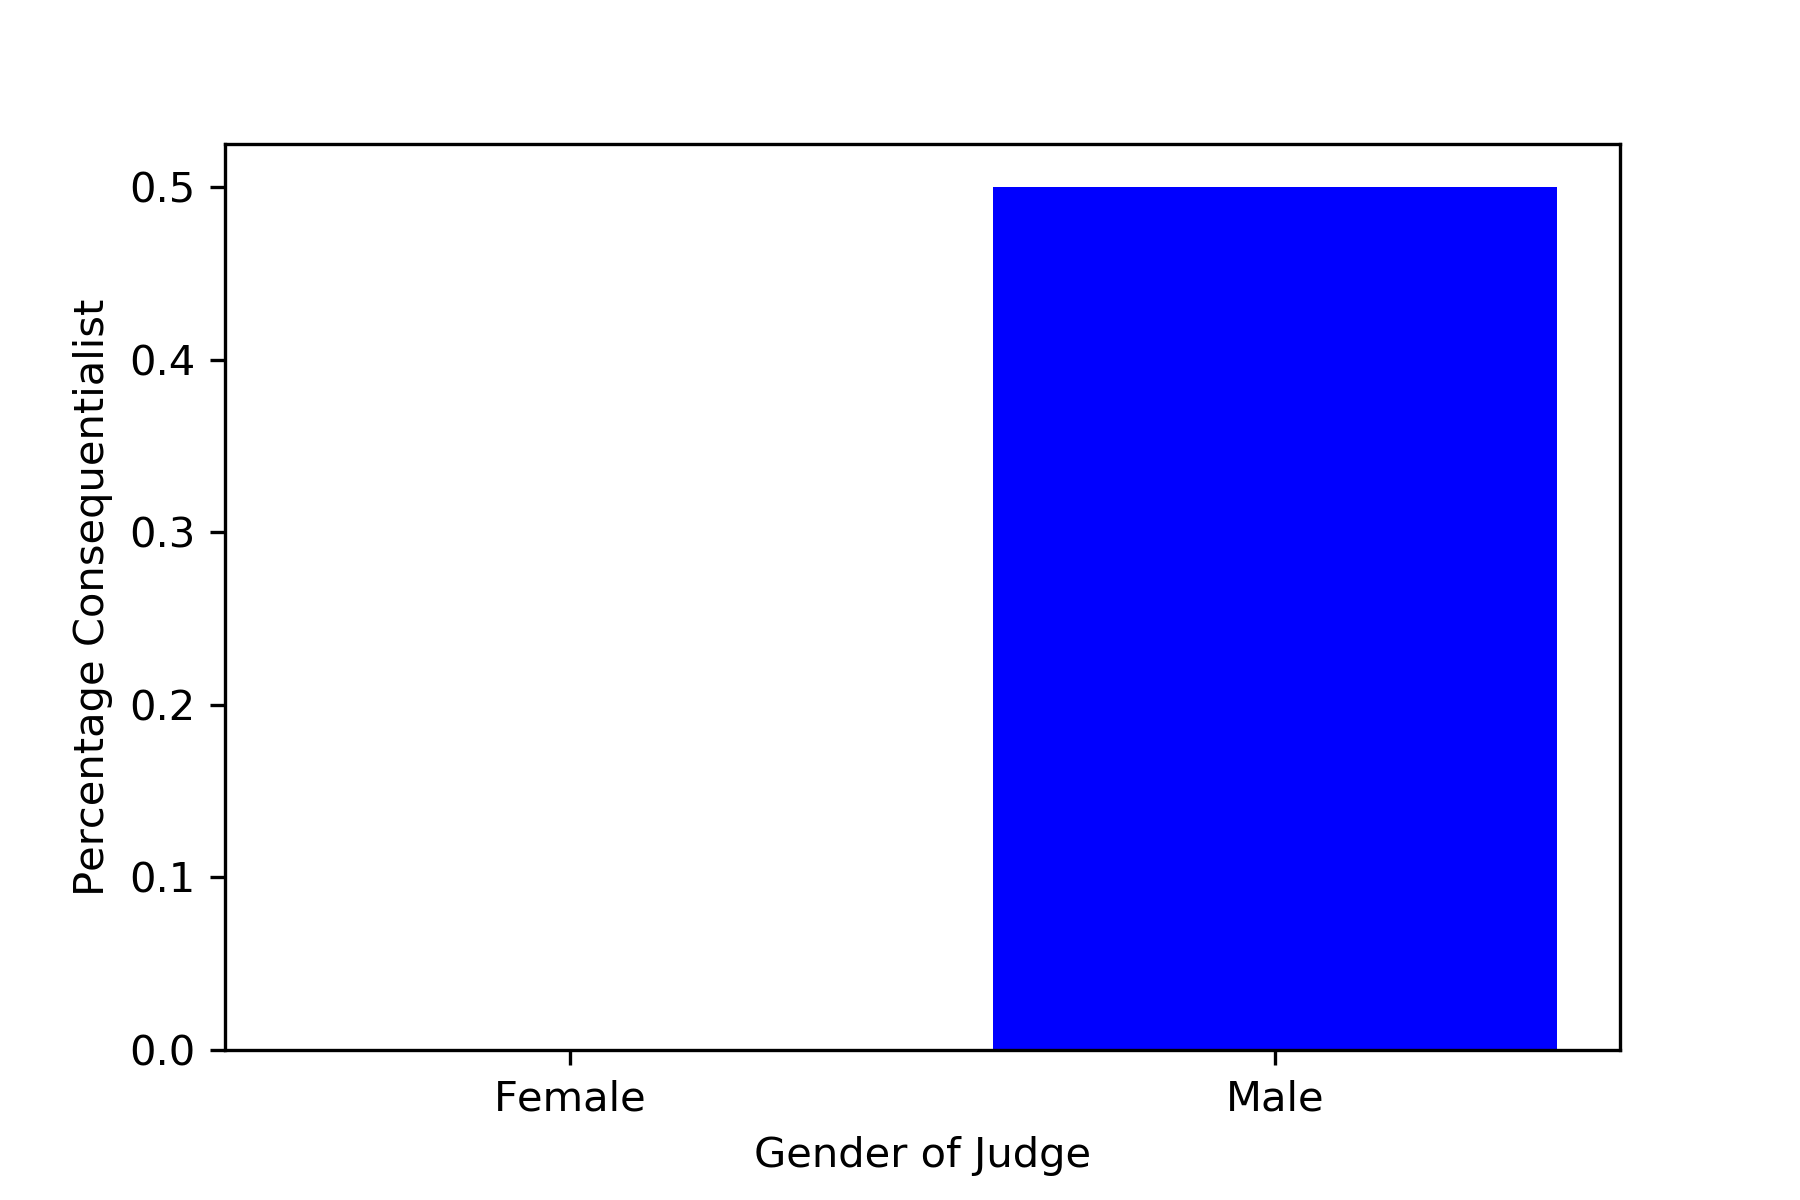
\includegraphics[width = 12cm, height = 8cm]{genderbar.png}
    \[\texttt{Bar Graph for Consequentialist reasoning by Gender}\]
\end{center}

\subsection{Consequentialist approach per Political Affiliation of the President}

There appears to be almost no difference in consequentialist reasoning across party affiliations of the President who appointed the judge.

\begin{center}
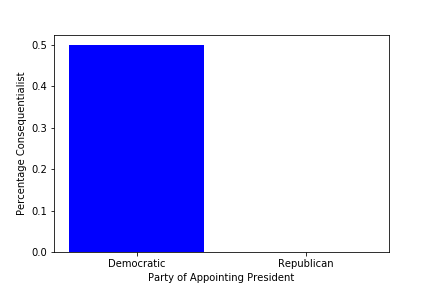
\includegraphics[width = 12cm, height = 8cm]{party.png}
    \[\texttt{Bar Graph for Consequentialist reasoning by Political affiliationa}\]
\end{center}

\subsection{Percentage Consequentialism by Birth States}

\begin{center}
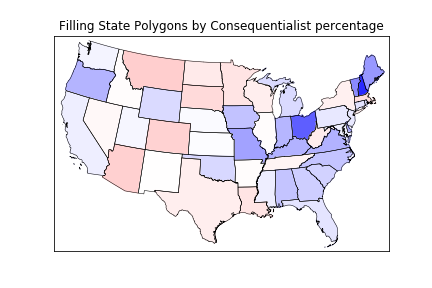
\includegraphics[width = 12cm, height = 8cm]{map.png}
    \[\texttt{Heat Map for Consequentialist reasoning by State. The more red, the more consequentialist of reasoning}\]
\end{center}







ADD: Another graph on a different data set
do a word cloud




\newpage

\subsubsection*{Acknowledgments}

Use unnumbered third level headings for the acknowledgments. All
acknowledgments go at the end of the paper. Do not include
acknowledgments in the annonymized submission, only in the final paper.

\section*{References}

References follow the acknowledgments. Use unnumbered first-level
heading for the references. Any choice of citation style is acceptable
as long as you are consistent. It is permissible to reduce the font
size to \verb+small+ (9 point) when listing the references. {\bf
  Remember that you can use a ninth page as long as it contains
  \emph{only} cited references.}
\medskip

\small

[1] Alexander, J.A.\ \& Mozer, M.C.\ (1995) Template-based algorithms
for connectionist rule extraction. In G.\ Tesauro, D.S.\ Touretzky and
T.K.\ Leen (eds.), {\it Advances in Neural Information Processing
  Systems 7}, pp.\ 609--616. Cambridge, MA: MIT Press.

[2] Bower, J.M.\ \& Beeman, D.\ (1995) {\it The Book of GENESIS:
  Exploring Realistic Neural Models with the GEneral NEural SImulation
  System.}  New York: TELOS/Springer--Verlag.

[3] Hasselmo, M.E., Schnell, E.\ \& Barkai, E.\ (1995) Dynamics of
learning and recall at excitatory recurrent synapses and cholinergic
modulation in rat hippocampal region CA3. {\it Journal of
  Neuroscience} {\bf 15}(7):5249-5262.

\end{document}